%%%%%%%%%%%%%%%%%%%%%%%%%%%%%%%%%%%%%%%%%
% Journal Article
% LaTeX Template
% Version 1.4 (15/5/16)
%
% This template has been downloaded from:
% http://www.LaTeXTemplates.com
%
% Original author:
% Frits Wenneker (http://www.howtotex.com) with extensive modifications by
% Vel (vel@LaTeXTemplates.com)
%
% License:
% CC BY-NC-SA 3.0 (http://creativecommons.org/licenses/by-nc-sa/3.0/)
%
%%%%%%%%%%%%%%%%%%%%%%%%%%%%%%%%%%%%%%%%%

%----------------------------------------------------------------------------------------
%	PACOTES E OUTRAS CONFIGURACOES DO DOCUMENTO
%----------------------------------------------------------------------------------------

\documentclass[
	twoside,				% frete e versohttps://preview.overleaf.com/public/dfmtjmgfyjgv/images/794855a0282c944a91303ddfdf56e0175d06e342.jpeg
	twocolumn,				% coluna dupla
	english,				% idioma adicional para hifenização
	brazil,					% o último idioma é o principal do documento
]{article}

% ---
% PACOTES
% ---

% ---
% Pacotes fundamentais 
% ---
\usepackage{cmap}			% Mapear caracteres especiais no PDF
\usepackage{lmodern}		% Usa a fonte Latin Modern			
\usepackage[T1]{fontenc}	% Selecao de codigos de fonte.
\usepackage[utf8]{inputenc}	% Codificacao do documento (conversão automática dos acentos)
\usepackage{indentfirst}	% Indenta o primeiro parágrafo de cada seção.
\usepackage{color}			% Controle das cores
\usepackage{graphicx}		% Inclusão de gráficos
\usepackage{lipsum}			% para geração de dummy text
\usepackage{blindtext}		% Package to generate dummy text throughout this template 
\usepackage{amsmath}

\usepackage[sc]{mathpazo}	% Use the Palatino font
\usepackage[T1]{fontenc}	% Use 8-bit encoding that has 256 glyphs
\linespread{1.05}			% Line spacing - Palatino needs more space between lines
\usepackage{microtype}		% Slightly tweak font spacing for aesthetics

\usepackage[brazil]{babel}	% Hifenizacao textual de regras tipograficas em portugues

\usepackage[hmarginratio=1:1,top=32mm,columnsep=20pt]{geometry} % Document margins
\usepackage[hang, small,labelfont=bf,up,textfont=it,up]{caption} % Custom captions under/above floats in tables or figures
\usepackage{booktabs} % Horizontal rules in tables

\usepackage{lettrine} % The lettrine is the first enlarged letter at the beginning of the text

\usepackage{enumitem} % Customized lists
\setlist[itemize]{noitemsep} % Make itemize lists more compact

\usepackage{abstract} % Allows abstract customization
\renewcommand{\abstractnamefont}{\normalfont\bfseries} % Set the "Abstract" text to bold
\renewcommand{\abstracttextfont}{\normalfont\small\itshape} % Set the abstract itself to small italic text

\usepackage{titlesec} % Allows customization of titles
\renewcommand\thesection{\Roman{section}} % Roman numerals for the sections
\renewcommand\thesubsection{\roman{subsection}} % roman numerals for subsections
\titleformat{\section}[block]{\large\scshape\centering}{\thesection.}{1em}{} % Change the look of the section titles
\titleformat{\subsection}[block]{\large}{\thesubsection.}{1em}{} % Change the look of the section titles

\usepackage{fancyhdr} % Headers and footers
\pagestyle{fancy} % All pages have headers and footers
\fancyhead{} % Blank out the default header
\fancyfoot{} % Blank out the default footer
\fancyhead[C]{Implementação de um controlador \textit{fuzzy} para um sistema de taques acoplados $\bullet$ Outubro 2016} % Custom header text
\fancyfoot[RO,LE]{\thepage} % Custom footer text

\usepackage{titling} % Customizing the title section

\usepackage{hyperref} % For hyperlinks in the PDF

%----------------------------------------------------------------------------------------
%	TITULO DA SECAO
%----------------------------------------------------------------------------------------

\setlength{\droptitle}{-4\baselineskip} % Move the title up

\pretitle{\begin{center}\Huge\bfseries} % Article title formatting
\posttitle{\end{center}} % Article title closing formatting
\title{Implementação de um Controlador Fuzzy para um sistema de taques acoplados: um estudo de caso.}
\author{
\textit{Fernando Fernandes}\thanks{\textbf{Fernando Fernandes}, Departamento de Computação e Automação, Centro de Tecnologia. \href{mailto:leandes@gmail.com}{leandes@gmail.com}} / 
\textit{Tiago Batista}\thanks{\textbf{Tiago Batista}, Departamento de Computação e Automação, Centro de Tecnologia. \href{mailto:ekyidag@gmail.com}{ekyidag@gmail.com}} / 
\textit{Rosenildo Pereira}\thanks{\textbf{Rosenildo Pereira}, Departamento de Computação e Automação, Centro de Tecnologia. \href{mailto:reidesgm@hotmail.com}{reidesgm@hotmail.com}} \\ [1ex]
\textsc{Universidade Federal do Rio Grande do Norte} \\
}
\date{\today} % Leave empty to omit a date
\renewcommand{\maketitlehookd}{%
\begin{abstract}
\noindent Este estudo aborda de configuração de um controlador PID \textit{fuzzy} utilizando os modelos de Sugeno e Mamdani para o controle de um sistema de tanques acoplados. Esta atividade foi desenvolvida utilizando o toolbox Fuzzy do Matlab R2016a Student e um modelo fornecido do Simulink. O objetivo do estudo é obter parâmetros de operação ótimos para o controlador PID dadas as condições de operação, considerando o erro entre o setpoint e o nível presente na planta, bem como a variação desse erro. Esta atividade foi proposta pelo Professor Dr. Fábio Meneghetti no escopo do componente Controle Fuzzy de Sistemas Dinâmicos do curso de Engenharia Mecatrônica da Universidade Federal do Rio Grande do Norte.
\end{abstract}
}

%----------------------------------------------------------------------------------------

\begin{document}

% Titulo do artigo
\maketitle

%----------------------------------------------------------------------------------------
%	CONTEUDO DO ARTIGO
%----------------------------------------------------------------------------------------

\section{Introdução}
\lettrine[nindent=0em,lines=3]{A} teoria dos conjuntos \textit{fuzzy}, idealizada em 1965 pelo matemático e pesquisador das área de ciência da computação, engenharia elétrica e inteligência artificial, o azerbaijano Lotfali Askar-Zadeh, é o alicerce da teoria que modela sistemas que lidam com dados e regras imprecisas. Assim como as pessoas o fazem cotidianamente.

A partir desse conceito, todo um conjunto de técnicas e tecnologias que fazem uso de definições linguísticas para o tratamento das informações e das ações de controle foi desenvolvida e estão presentes virtualmente em qualquer aparelho que necessite realizar inferências de controle mais refinadas que o simples controle \textit{on/off}.

Controladores \textit{fuzzy} atualmente ocupam posição de destaque entre as técnicas de controle empregadas na indústria, ainda superada, em quantidade, apenas pelo controle PID clássico.

(Organização do artigo)
%------------------------------------------------

\section{Revisão de Conceitos}

As primeiras aplicações de algoritmos \textit{fuzzy} em problemas de controle foi trabalho pioneiro de \cite{Mamdani:1973}, seguido por \cite{Sugeno:1985}, ambos motivados pelos trabalhos de \cite{Zadeh:1965} e \cite{Zadeh:1973}. \cite{TakagiSugeno:1983}, observando dificuldades para a implementação do processo de decisão do controlador de Mamdani, propuseram um método de tomada de decisão simplificado, baseado na lógica \textit{fuzzy}, onde somente o antecedente das regras é formado por variáveis \textit{fuzzy}. O conseqüente de cada regra é expresso por uma função linear dos valores observados das variáveis que descrevem o estado do sistema (variáveis de entrada). Este tipo de controlador é referido na literatura como controlador de Sugeno (Lee, 1990a; Zimmermann, 1996; MathWorks, 2008).

Controladores aprimorados de Mamdani e Sugeno sofreram têm sido utilizados para diferentes aplicações (Lee, 1990a). Atualmente estão disponíveis em pacotes computacionais, com diferentes recursos para implementação dos seus componentes, o que facilita o desenvolvimento de controladores \textit{fuzzy} para a solução de diferentes problemas de controle. A escolha do tipo de controlador a adotar e a forma de implementação dos seus diferentes componentes, exige do projetista conhecimento dos aspectos teóricos envolvidos em cada solução e, além disso, razoável noção do impacto de cada escolha (tipo de controlador e implementação dos componentes) sobre a eficácia do controle por ele produzido.

No controlador desenvolvido foi adotado um método para o processo de decisão baseado em regras do tipo “SE A ENTÃO B”, nas quais tanto o antecedente quanto o conseqüente são valores de variáveis lingüísticas, expressos por meio de conjuntos \textit{fuzzy} (Mamdani e Assilian, 1975). 

%------------------------------------------------

\section{Modelos de Controladores \textit{Fuzzy}}

\textit{Os controladores fuzzy descritos na literatura são classificados em função das características gerais do seu método de tomada de decisão. Embora diferentes métodos sejam apresentados na literatura (ver Lee, 1990b), de acordo com Sugeno (1985) eles podem ser reunidos em dois grandes grupos. O primeiro reúne os que são baseados nas funções de implicação fuzzy e em operadores de composição para a definição da saída fuzzy do controlador. Já os do segundo grupo dispensam a definição de funções de implicação e operadores para a inferência. Os controladores do tipo Mamdani, referidos nesta seção como controlador de Mamdani, são baseados no primeiro grupo, e os controladores do tipo desenvolvido por Takagi e Sugeno, aqui referidos como controlador de Sugeno, fazem parte do segundo grupo.}

\textit{Nos dois tipos de controladores a ação de controle é obtida por meio da definição de um conjunto de instruções (ou regras) de controle fuzzy, isto é de um algoritmo fuzzy. Essas regras são do tipo GMP (\textit{Generalized Modus Ponens}), e uma dada regra (Ri) pode ser apresentada como:}
$$
Antecedente: x é A’ e y é B’ 
Regra (R i ): se x é A i e y é B i então z é C i 
Conseqüente: z é C’ i 
$$
\textit{onde x and y são variáveis lingüísticas relacionadas ao estado do processo e z é a variável lingüística de controle; A’, A i , B’, B i , C’ i e Ci são conjuntos \textit{fuzzy} de x, y e z nos universos de discurso U, V e W, respectivamente. Como será apresentado a seguir, no caso do controlador de Sugeno, o conseqüente da regra não é um conjunto \textit{fuzzy}.}


\subsection{Controlador Mamdani}

\textit{Este controlador tem como base o trabalho pioneiro de Mamdani, publicado em 1973 (Mamdani, 1973). No algoritmo fuzzy do controlador, cada regra é uma proposição condicional fuzzy, e diferentes relações fuzzy em U x V x W podem ser dela derivadas.
A implementação de cada regra é feita mediante a definição de operadores para o processamento do antecedente da regra e da função de implicação que irá definir o seu conseqüente. A ação do controlador fuzzy é definida pela agregação das n regras R i que compõem o algoritmo, mediante o uso do conectivo “também”, o qual pode ser implementado por diferentes operadores. Esta agregação resulta no conjunto fuzzy C, que define a saída do controlador C. A saída efetiva do controlador é então obtida por meio de um processo de defuzificação aplicado ao conjunto C.}

\textit{As diferentes possibilidades para a implementação dos conectores das regras, das funções de implicação e do processo de defuzificação são amplamente discutidas na literatura (ver, por exemplo, Lee 1990a e 1990b) e não serão tratadas no presente trabalho. O impacto da adoção de algumas dessas possibilidades, e da definição dos conjuntos fuzzy associados às variáveis de entrada do controlador semafórico fuzzy, foram objeto de pesquisas anteriores (Jacques et al., 2002b, 2002c, 2003; Vaz, 2006)}

\subsection{Controlador Sugeno}

\textit{O controlador de Sugeno (Takagi e Sugeno, 1983) consiste numa simplificação do controlador de Mamdani, onde o conseqüente de cada regra é definido como uma função das variáveis lingüísticas de entrada. Isto é, a regra geral R i pode ser escrita como:}
$$
Regra (R i ): se x é A i e y é B i então z = f i (x, y)
$$
\textit{O resultado de cada regra é, portanto, um valor numérico (não um conjunto fuzzy), que assume como peso o valor da pertinência resultante do processamento do antecedente da regra. Essa determinação dispensa, portanto, a definição de uma função de implicação específica. A resposta final do controlador é obtida pela média ponderada das respostas das regras individuais. Isto é, neste tipo de controlador não cabe processo de defuzificação.}

\textit{O valor de z pode também ser definido como um valor constante, que pode ser interpretado como um conjunto fuzzy com a característica especial de apresentar um único valor com pertinência igual a um e todos os demais com pertinência zero. Este tipo de conjunto fuzzy é denominado singleton, e o seu emprego permite a definição de regras com valores de saída que representam uma classificação da resposta do controlador, sem alterar a forma simplificada da determinação da resposta final do controlador.}

\subsection{Implementação computacional}

\textit{A implementação de um controlador fuzzy, para fins de utilização efetiva,  equer o uso de programas computacionais. Atualmente, alguns programas de uso geral dispõem de módulos específicos para facilitar a realização desta tarefa, como é o caso do Fuzzy Logic Toolbox do MATLAB \textsuperscript{\textregistered}, usado neste trabalho para implementar os dois tipos de controladores em estudo. O programa permite ao usuário definir os quatro componentes principais do sistema de inferência fuzzy, que são: fuzificação dos valores das variáveis de entrada e aplicação dos operadores que podem estar presentes no antecedente das regras (“e” e “ou”); implicação do antecedente sobre o conseqüente (função de implicação); agregação dos conseqüentes de todas as regras definidas; e a defuzificação do conjunto C de resposta. No MATLAB\textsuperscript{\textregistered} , antes de iniciar a definição dos componentes do sistema, o usuário deve indicar se o seu controlador é do tipo Mamadani ou Sugeno. Dependendo do tipo selecionado, são liberados os campos pertinentes para a entrada dos dados. Isto é, se for selecionado o controlador de Sugeno, por exemplo, os campos referentes à função de implicação, ao termo de agregação “também” e ao método de defuzificação ficam desabilitados. O programa apresenta diferentes opções ao usuário para a configuração dos componentes do sistema e, para a maioria dos campos, também permite a definição de outras alternativas. }

\section{O problema}

O sistema a ser controlado é o sistema de tanques acoplados da Quanser\textsuperscript{\textregistered}, que tem model matemático dado por:
\begin{equation}
\label{eq:dL1}
\dot{L_{1}} = - \frac{a_{1}}{A_{1}} \sqrt{\frac{g}{2L_{1o}}}L_{1}+\frac{K_{m1}}{A_{1}}V_{p1}
\end{equation}

\begin{equation}
\label{eq:dL2}
\dot{L_{2}} = - \frac{a_{2}}{A_{2}} \sqrt{\frac{g}{2L_{2o}}}L_{2}+\frac{a_{1}}{A_{1}} \sqrt{\frac{g}{2L_{1o}}}L_{1}
\end{equation}

Onde $L_{1}$ e $\dot{L_{1}}$ são o nível do tanque superior e sua variação. O mesmo vale para $L_{2}$ e $\dot{L_{2}}$, para o tanque inferior. As constantes $a_{1}$ e $A_{1}$, assim como $a_{2}$ e $A_{2}$, são as áreas dos orifícios e da seção transversal dos tanques superior e inferior, respectivamente. $V_{p1}$ é a tensão aplicada à bomba e $K_{m1}$ é a constante da bomba. Discretizando o modelo para o período de amostragem da planta (100 ms) e aplicando as constantes fornecidas pelo fabricante do experimento temos:

\begin{equation}
\label{eq:discrete}
\begin{cases}
L_{1}(k) = 0,9935 L_{1}(k-1) + 0,0296V_{p1}(k-1) \\
L_{2}(k) = 0,0065L_{1}(k-1)+0,9935L_{2}(k-1)+ \\ 
\hspace{1.33cm}0,0001V_{p1}(k-1)
\end{cases}
\end{equation}

\section{Metodologia}

De forma suscinta, as funções de pertinência foram incialmente escolhidas empiricamente e refinadas conforme foram sendo realizadas as simulações e observado o comportamento do sistema. Baseado nas funções de pertinência definidas foi construída o conjunto de regras de inferência, considerando a quantidade de entradas e funções. Em sequência, definiram-se as funções lineares de pertinência da saída, a saber:

\itemize{
\item{MANTER: ação fraca para manutenção do nível do tanque quando nível está próximo ao \textit{setpoint}.}
\item{SUBIR: ação moderada para aumento do nível do tanque quando o nível do tanque está abaixo do \textit{setpoint}, mas convergindo para ele.}
\item{DESCER: ação moderada para redução do nível do tanque quando o nível do tanque está acima do \textit{setpoint}, mas convergindo para ele.}
\item{SUBIR FORTE: ação intensa para aumento do nível do tanque quando o nível está divergindo decrescentemente do \textit{setpoint}.}
\item{DESCER FORTE: ação intensa para redução do nível do tanque quando o nível está divergindo crescentemente do \textit{setpoint}.}
}

O parâmetros de controle definidos para cada umas das funções de saída, expresso por um vetor de saída com 3 elementos, onde o primeiro comporta-se como o fator integrativo, o segundo como o proporcional e o terceiro como uma constante de offset do modelo clássico da teoria de controle. Os valores foram escolhidos pela observação do comportamento da simulação.

\subsection{Modelo Sugeno}

Mesmo com a saturação do sinal da bomba, limitado a $\pm4$, o overshoot somente foi sanado com a ação da integração do erro quando o sinal da bomba entrava em saturação. Esta técnica é documentada na literatura como \textit{anti-windup}\footnote{refrências podem ser enconradas em: \ldots}.

A determinação dos parâmetros proporcional, integrativo e da constante foi feita de forma empírica.

\subsection{Modelo Mamdani}

A escolhas das regras seguiu os mesmos procedimentos do Sugeno, com exceção da saída que tem três funções de pertinência triangulares (MANTER, SUBIR E DESCER), nos quais definiram-se os valores de incremento do sinal de controle.

Foram realizados dois testes. Um com as funções de saída simétricas e funções de pertinência do erro deslocadas para a esquerda para compensar a vazão dos orifícios de saída dos tanques (teste 1). O segundo teste foi feito o inverso, as funcções de pertinência do erro foram simétricas e as funões de saída foram deslocadas à direita para, novamente, estabilizar o nível do tanque compensando a vazão de saída (teste 2). O terceiro teste foi feito deslocando as funções de pertinência do erro para a esquerda e as funões de saída foram deslocadas à direita para, novamente, estabilizar o nível do tanque compensando a vazão de saída (teste 3).

\section{Resultados}

\begin{table}
\caption{Regras para do controlador Sugeno}
\centering
\begin{tabular}{lllr}
\toprule
\multicolumn{3}{r}{\textbf{Erro}} \\
\cmidrule(r){2-4}
\textbf{Derivada} & \textbf{Negativo} & \textbf{Nulo} & \textbf{Positivo} \\
Negativa & Descer & Manter & Subir \\
Nula & Descer & Manter & Subir \\
Positiva & Descer & Manter & Subir \\
\bottomrule
\end{tabular}
\end{table}

\begin{table}
\caption{Parâmetros de configuração para o controlador Sugeno (5)}
\centering
\begin{tabular}{llll}
\toprule
\multicolumn{2}{c}{\textbf{Erro e Derivada}} & \multicolumn{2}{c}{\textbf{Saída}}  \\
\midrule
\textbf{EN} & [-4970  -4970  -8  -1] & \textbf{SF} & [0.1 10 0] \\
\textbf{EZ} & [-3 0 1] & \textbf{S} & [0.09 1.5 0] \\
\textbf{EP} & [0 6 30 5500] & \textbf{M} & [0.05 1 0] \\
\textbf{VEN} & [-2  -1 0.104] & \textbf{D} & [0.08 3 0] \\
\textbf{VEZ} & [-0.2 0 0.1] & \textbf{DF} & [0.05 2.5 0] \\
\textbf{VEP} & [0 1 2] & & \\
\bottomrule
\end{tabular}
\end{table}

\includegraphics[width=\columnwidth]{sugeno5}

\begin{table}[htbp]
\caption{Parâmetros de comparação para configuração para o controlador Sugeno (1) - melhor resultado}
\centering
\begin{tabular}{llll}
\toprule
\multicolumn{2}{c}{\textbf{Erro e Derivada}} & \multicolumn{2}{c}{\textbf{Saída}}  \\
\midrule
\textbf{EN} & [-543  -87  -15  -3.5] & \textbf{SF} & [0.5 10 0] \\
\textbf{EZ} & [-5 -1.15 3] & \textbf{S} & [0.3 10 0] \\
\textbf{EP} & [2 15 87 543] & \textbf{M} & [0.045 1.4 0] \\
\textbf{VEN} & [-10  -1  -0.08] & \textbf{D} & [0.3 3.5 0] \\
\textbf{VEZ} & [-0.15 0 0.08] & \textbf{DF} & [0.1 1.5 0] \\
\textbf{VEP} & [0.06 1 5] & & \\
\bottomrule
\end{tabular}
\end{table}

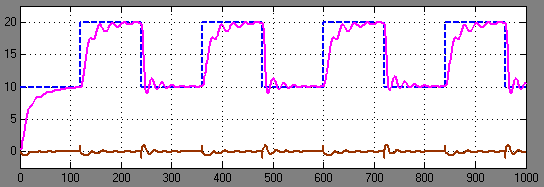
\includegraphics[width=\columnwidth]{sugeno1}

\begin{table}
\caption{Parâmetros de comparação para configuração para o controlador Sugeno (3)}
\centering
\begin{tabular}{llll}
\toprule
\multicolumn{2}{c}{\textbf{Erro e Derivada}} & \multicolumn{2}{c}{\textbf{Saída}}  \\
\midrule
\textbf{EN} & [-4970 -4970 -10 -1] & \textbf{SF} & [0.05 10 0] \\
\textbf{EZ} & [-5 0 5] & \textbf{S} & [0.18 3 0] \\
\textbf{EP} & [1 10 30 5500] & \textbf{M} & [0.04 0.55 0] \\
\textbf{VEN} & [-2 -1 -0.104] & \textbf{D} & [0.08 2 0] \\
\textbf{VEZ} & [-0.2 0 0.2] & \textbf{DF} & [0.05 2.5 0] \\
\textbf{VEP} & [0 1 2] & & \\
\bottomrule
\end{tabular}
\end{table}

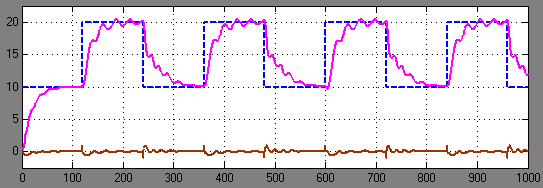
\includegraphics[width=\columnwidth]{sugeno3}

% \begin{table}
% \caption{Example table}
% \centering
% \begin{tabular}{llr}
% \toprule
% \multicolumn{2}{c}{Name} \\
% \cmidrule(r){1-2}
% First name & Last Name & Grade \\
% \midrule
% John & Doe & $7.5$ \\
% Richard & Miles & $2$ \\
% \bottomrule
% \end{tabular}
% \end{table}

%------------------------------------------------

\section{Discussão}

\subsection{Subsection One}

A statement requiring citation \cite{Figueredo:2009dg}.

\subsection{Subsection Two}

%----------------------------------------------------------------------------------------
%	REFERENCIAS
%----------------------------------------------------------------------------------------

\begin{thebibliography}{99} % Bibliography 

\bibitem[Mamdani, 1973]{Mamdani:1973}
Mamdani, E. H. e Assilian S. (1973)
\newblock Aplications of fuzzy algorithms for control of simple dynamic plant.
\newblock {\em Proc. IEEE 121}, vol. 12, p. 1585-1588.

\bibitem[Mamdani, 1975]{Mamdani:1975}
Mamdani, E. H. e Assilian S. (1975)
\newblock An experiment in linguistic synthesis with a fuzzy logic controller.
\newblock {\em International Journal Man-Machine Studies}, vol. 7, p. 1-13.

\bibitem[Takagi e Sugeno, 1983]{TakagiSugeno:1983}
Takagi, T. e Sugeno M. (1983).
\newblock Derivation of fuzzy control rules from human operator’s control action.
\newblock {\em IFAC Symposium on Fuzzy Information, Knowledge Representation and Decision Analysis}, Marseille, p. 55-60.

\bibitem[Zadeh, 1973]{Zadeh:1973}
Zadeh, L. A. (1973).
\newblock Outline of a new approach to the analysis of complex systems and decision processes.
\newblock {\em IEEE Transactions on Systems, Man, and Cybernetics}, Vol. SMC-3, No. 1, p. 28-44.

\end{thebibliography}

%----------------------------------------------------------------------------------------

\end{document}
